\documentclass{beamer}\usepackage{graphicx, color}
%% maxwidth is the original width if it is less than linewidth
%% otherwise use linewidth (to make sure the graphics do not exceed the margin)
\makeatletter
\def\maxwidth{ %
  \ifdim\Gin@nat@width>\linewidth
    \linewidth
  \else
    \Gin@nat@width
  \fi
}
\makeatother

\IfFileExists{upquote.sty}{\usepackage{upquote}}{}
\definecolor{fgcolor}{rgb}{0.2, 0.2, 0.2}
\newcommand{\hlnumber}[1]{\textcolor[rgb]{0,0,0}{#1}}%
\newcommand{\hlfunctioncall}[1]{\textcolor[rgb]{0.501960784313725,0,0.329411764705882}{\textbf{#1}}}%
\newcommand{\hlstring}[1]{\textcolor[rgb]{0.6,0.6,1}{#1}}%
\newcommand{\hlkeyword}[1]{\textcolor[rgb]{0,0,0}{\textbf{#1}}}%
\newcommand{\hlargument}[1]{\textcolor[rgb]{0.690196078431373,0.250980392156863,0.0196078431372549}{#1}}%
\newcommand{\hlcomment}[1]{\textcolor[rgb]{0.180392156862745,0.6,0.341176470588235}{#1}}%
\newcommand{\hlroxygencomment}[1]{\textcolor[rgb]{0.43921568627451,0.47843137254902,0.701960784313725}{#1}}%
\newcommand{\hlformalargs}[1]{\textcolor[rgb]{0.690196078431373,0.250980392156863,0.0196078431372549}{#1}}%
\newcommand{\hleqformalargs}[1]{\textcolor[rgb]{0.690196078431373,0.250980392156863,0.0196078431372549}{#1}}%
\newcommand{\hlassignement}[1]{\textcolor[rgb]{0,0,0}{\textbf{#1}}}%
\newcommand{\hlpackage}[1]{\textcolor[rgb]{0.588235294117647,0.709803921568627,0.145098039215686}{#1}}%
\newcommand{\hlslot}[1]{\textit{#1}}%
\newcommand{\hlsymbol}[1]{\textcolor[rgb]{0,0,0}{#1}}%
\newcommand{\hlprompt}[1]{\textcolor[rgb]{0.2,0.2,0.2}{#1}}%

\usepackage{framed}
\makeatletter
\newenvironment{kframe}{%
 \def\at@end@of@kframe{}%
 \ifinner\ifhmode%
  \def\at@end@of@kframe{\end{minipage}}%
  \begin{minipage}{\columnwidth}%
 \fi\fi%
 \def\FrameCommand##1{\hskip\@totalleftmargin \hskip-\fboxsep
 \colorbox{shadecolor}{##1}\hskip-\fboxsep
     % There is no \\@totalrightmargin, so:
     \hskip-\linewidth \hskip-\@totalleftmargin \hskip\columnwidth}%
 \MakeFramed {\advance\hsize-\width
   \@totalleftmargin\z@ \linewidth\hsize
   \@setminipage}}%
 {\par\unskip\endMakeFramed%
 \at@end@of@kframe}
\makeatother

\definecolor{shadecolor}{rgb}{.97, .97, .97}
\definecolor{messagecolor}{rgb}{0, 0, 0}
\definecolor{warningcolor}{rgb}{1, 0, 1}
\definecolor{errorcolor}{rgb}{1, 0, 0}
\newenvironment{knitrout}{}{} % an empty environment to be redefined in TeX

\usepackage{alltt}
\usetheme{Stats}
\setbeamercovered{transparent}
\usepackage{color}
\usepackage{hyperref}
  \hypersetup{
  	colorlinks=true
		linkcolor=black
		}
\usepackage{url}
\usepackage{graphics}
\usepackage{tikz}
\usepackage{booktabs}





%%%%%%%%%%%%%%%%%%%%%%%%%%%%%%%% Title Slide %%%%%%%%%%%%%%%%%%%%%%%%%%
\title[]{Intro to Social Science Data Analysis \\[1cm] Seminar 6: Data Visualisation in R}
\author[]{
    \href{mailto:gandrud@yonsei.ac.kr}{Christopher Gandrud}
}
\date{\today}


\begin{document}

\frame{\titlepage}

\frame{
	\frametitle{Principles of Graphical Excellence}
  What does it mean to ``show the data"? \\[0.5cm]
  What is a high data-ink ratio?
}

\frame{
  \frametitle{What's the story? How well does the graph help you see it? How could it be better?}
  \begin{center}
    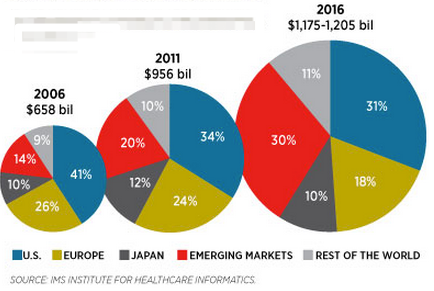
\includegraphics[scale=0.6]{CircleTerror.png}
  \end{center}
}

\frame{
  \frametitle{Better}
  \begin{center}
    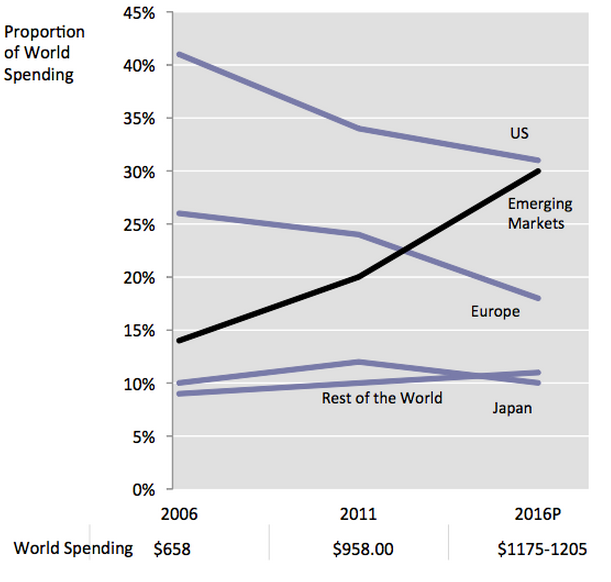
\includegraphics[scale=0.35]{NoMoreCircleTerror.png} \\
    {\tiny{Source: \url{http://junkcharts.typepad.com/junk_charts/2012/10/expanding-circles-of-error.html}}}
  \end{center}
}

\frame{
  \frametitle{Base R Graphics}
  Make a graph in base R (using any data). \\[0.25cm]
  Make sure the figure is labeled well.
}

\frame{
  \frametitle{ggplot2}
  With ggplot2 make: 
  \begin{itemize}
    \item A scatter plot,
    \item A density plot
    \item A line graph 
    \item A bar graph
  \end{itemize}\\[0.25cm]
  Use colour to show groups in your data in at least one of these graphs.
}


\frame{
  \frametitle{Maps}
  Make a map with googleVis,
}

\frame{
  \frametitle{Assignment 2}
  \textbf{Due:} Friday 19 October \\[0.25cm]
  
  \textbf{Describe} at least \textbf{3} variables in a data set.\\[0.25cm]
  {\small{
    You need to select a \textbf{range of descriptive statistical tools}. The tools should include both \textbf{numerical descriptive statistics} and \textbf{graphics}.\\[0.25cm]

    These tools should describe the variables':
    \begin{itemize}
      \item<1-> central tendency,
      \item<1-> variation,
      \item<1-> their relationships with the other variables.
    \end{itemize}

    The descriptions need to be discussed \textbf{in paragraph form}. \\[0.25cm]

    The description must be \textbf{reproducible}. So you should email me the link to a Dropbox folder with:
    \begin{itemize}
      \item<1-> the \texttt{.csv} data set,
      \item<1-> the \texttt{.Rmd} R markdown file,
      \item<1-> the final \texttt{.html} file.
    \end{itemize}
  }}
}


\end{document}
